%% Template for a preprint Letter or Article for submission
%% to the journal Nature.
%% Written by Peter Czoschke, 26 February 2004
%%

\documentclass{nature}

\usepackage[
active,
generate=Abstract_excerpt,
extract-env=figure
]{extract}

%% make sure you have the nature.cls and naturemag.bst files where
%% LaTeX can find them

\bibliographystyle{naturemag}
\usepackage[]{algorithm2e}

%\begin{extract}
% % KN, this next section restores inline images for the Nature template. Ok for first submission, remove for final submission.
\usepackage{graphicx}
\makeatletter
\let\saved@includegraphics\includegraphics
\AtBeginDocument{\let\includegraphics\saved@includegraphics}
\renewenvironment*{figure}{\@float{figure}}{\end@float}
\makeatother
%\end{extract}

\title{Urban typologies through city block size and regularity.}


%% Notice placement of commas and superscripts and use of &
%% in the author list

\author{Kerry~A.~Nice$^{1*}$,
Gideon D.P.A. Aschwanden$^{1*}$
%, Jasper S. Wijnands$^{1}$
%, Jason Thompson$^{1,2}$
%, Michele Acuto$^{1}$
%, Haifeng Zhao$^{1}$ \&
%, Mark Stevenson$^{1,3}$
}




\begin{document}




\maketitle

\begin{affiliations}
 \item Transport, Health, and Urban Design Hub, Faculty of Architecture, Building, and Planning, University of Melbourne, Victoria, Australia.
% \item Centre for Human Factors and Sociotechnical Systems, University of the Sunshine Coast, Australia.
% \item Melbourne School of Engineering; and Melbourne School of Population and Global Health, University of Melbourne, Victoria, Australia.
 \\ \textsuperscript{*} These authors contributed equally to this work
\end{affiliations}

%\begin{extract}
\begin{abstract}

%\begin{summary}
%\section{Summary}
% 150 words
% Motivation
Cities are a stage of human interactions, the foundation of society, a large source of pollution, and the habitat of the majority of the world's population. Although each field investigates cities from its own vantage point, we lack an objective method to compare cities around the world and therefore believe that each city is unique. This has led to repeated reinvention of solutions for problems that occur globally. Additionally, the lack of comparable measurement methods between and within cities starves us of the possibility to learn from previous examples.

% Solution
This paper presents a methodology that can reliably compare not only cities but individual neighbourhoods within cities in a robust manner using an unsupervised learning algorithms, a Self Organising Map (SOM), and map imagery created using a global dataset. The SOM projects n-dimensional spaces onto a 2-dimensional plane and can absorb additional data points and alternative data sets.
% Results
This allows us to identify similarities and patterns of precincts and urban structures across the globe. The findings show that city centres and suburban structures are objectively similar globally.
% Future
This method can now be deployed to find correlations with other indicators, to help planners and designers create a path to a desirable future and help manage and govern large urban entities by avoiding past pitfalls.


%\end{summary}

% City's 'uniqueness' 
As cities grow and evolve, analysis of the basic structural elements of road networks and urban blocks can provide clues as to the processes and governance under which city development occurred. The built environment has been shown to influence a wide range of outcomes, including health, transport, and economic opportunity. Methods to study cities through these basic structural elements are essential to many disciplines conducting urban research and provide a foundation on which they can conducting their research.
% Implication of city structure and form
 % and in particular / especially the road network and block typology,%


% our solution
We propose a novel, quantitative, and objective method to discover city typologies on a neighbourhood scale of street patterns by evaluating city block size and regularity. This follows Louf \& Barthelemy's finding\cite{Louf2014a} that a systematic quantitative method to identify different neighbourhoods is currently lacking. 
%% solution is globally applicabl | updates easily |  Robust | new city characteristics | can accomodate additonal data |
Our method uses imagery from Google Maps of custom, abstract, and stylized maps of ~400x400m sections of the world's largest 1667 cities. Using a  computer vision floodfill technique, the size and regularity of city blocks in the map samples are calculated and histogram representations constructed for each. A SOM is then used to sort the histograms, projecting the high dimensional space onto a 2-dimensional plane, revealing distinct city block typologies (see Figure \ref{fig:somresults}). 

% Results
%% Method is robust visible by global results
%% intra inter city similarities
%% Examples from Melbourne (and other cities)
The methodology has evaluated 1.7 million maps from 1667 cities, showing the robustness and global applicability of the methodology. The results of the SOM are used to colour code and highlight the map samples according to their SOM x,y coordinates. This process highlights similarities between city locations and has shown capable of detecting city archetypes such as city centres, suburban areas, and even more ephemeral entities such as the city edges (see Figure \ref{fig:mel23000}).
 
This method is not limited to detecting differences within a city, but is able to use a neighbourhood samples of one city and identify similar locations in all other cities. The global and heterogeneous collection of 1667 cities indicates the robustness of the methodology in classifying and identifying typologies in the respective map samples through the SOM (see Figure \ref{fig:world}).

% Maybe we should add a map segment of melbourne CBD and which other areas in the world are similar.


% Future Work
%% Find correlations with other indicators
Since this methodology promises to be applicable across many fields, the aim of future investigation(s) is to find correlations between urban typologies and other indicators. The potential candidates for such investigations are energy intensity, particular matter, and GDP since they are indicators that are globally available. The logical consequence is to test the methodology towards its predictive power and application in design, planning, and management of urban systems.


%For Nature, the abstract is really an introductory paragraph set
%in bold type.  This paragraph must be ``fully referenced'' and
%less than 180 words for Letters.  This is the thing that is
%supposed to be aimed at people from other disciplines and is
%arguably the most important part to getting your paper past the
%editors.  End this paragraph with a sentence like ``Here we
%show...'' or something similar.
\end{abstract}

\begin{figure}
\centering    
\includegraphics[scale=0.10]{Images/SomImages_grid.png}  
\caption{\bf  A visualisation of the 2-dimensional 100x100 SOM trained with 1.7 million map images from 1667 cities.  Each x,y point shows a representative image associated with each node while nodes without associated images are shown in black.}    
 \label{fig:somresults}  
\end{figure} 

\begin{figure}
\centering    
\includegraphics[scale=0.70,page=1]{Images/Melbourne_5_Final.pdf}  
\caption{\bf  Map of Melbourne, Australia with 24027 individual map segments classified and colour coded. Insert image on bottom left shows colour coding scheme for SOM x,y locations of Figure \ref{fig:somresults}. Note, the central business district (CBD) region shows additional points due to inclusion of the 1000 circular sampling procedure in addition to the 23,027 locations sampled at 400m resolution. }    
 \label{fig:mel23000}  
\end{figure} 


\begin{figure}
\centering    
\includegraphics[scale=0.85,page=1]{Images/Figure_3_World.pdf}  
\caption{\bf  1667 world cities sampled with inserts showing detail of (left) San Francisco, (centre) Nairobi, and (right) Tokyo. City detail maps use the same SOM x,y location colour scheme as Figure \ref{fig:mel23000}.}    
 \label{fig:world}  
\end{figure} 

%\end{extract}
% % Beginning of main text of the article

%Articles are original reports whose conclusions represent a substantial advance in understanding of an important problem and have immediate, far-reaching implications. They do not normally exceed 5 pages of Nature and, as a guideline, allow up to 50 references. (One page of undiluted text is about 1,300 words.) Articles have a summary, separate from the main text, of up to 150 words, which does not have references, and does not contain numbers, abbreviations, acronyms or measurements unless essential. It is aimed at readers outside the discipline. This summary contains a paragraph (2-3 sentences) of basic-level introduction to the field; a brief account of the background and rationale of the work; a statement of the main conclusions (introduced by the phrase 'Here we show' or its equivalent); and finally, 2-3 sentences putting the main findings into general context so it is clear how the results described in the paper have moved the field forwards. 

%Articles are typically 3,000 words of text, beginning with up to 500 words of referenced text expanding on the background to the work (some overlap with the summary is acceptable), before proceeding to a concise, focused account of the findings, ending with one or two short paragraphs of discussion. The text may contain a few short subheadings (not more than six in total) of no more than 40 characters each (less than one line of text in length). Articles typically have 5 or 6 display items (figures or tables).


%\section{Introduction}\label{sec:introduction}

%% Why is understanding the city so important
%% - Health (Lancet)
%% - Transport (Space Syntax)
%% - Economics (Urban Economics)

\subsection{City Typologies.}\label{sec:introduction2}
Cities are the most complex entities humans have ever created, but they are examples of `organised complexity' that allow us to discern some kind of order within the diversity and complexity cities present\cite{Kropf2014}. The form a city takes and the way land uses are allocated can have a detrimental impact on population health and well-being, including car dependency, physical inactivity, and associated illness such as obesity and road trauma\cite{Giles-corti2016, Kleinert2016, Goenka2016,Zapata-Diomedi2017, Heesch2014, Daley2011, Cepeda2016, MingWen2008, Norman2006, Thompson2018b}. Policy-makers and urban/transport planners have an opportunity to reverse this situation by embracing strategies that pro-actively support safe active transport modes as facilitated by urban designs witnessed in some countries around the world. However, understanding the association between urban design features, transport networks, or environmental outcomes remains difficult, especially when underlying data, locations, methods, and demographics upon which statistical models are built vary considerably. As a result, globally consistent comparisons between cities are difficult to achieve. 

Attempts to find quantitative methods, to create city typologies to assess, describe, and classify different types of urban form, have been under way for a number of decades. First attempts used broad demographics and functional characteristics to classify different types of cities. Occupational and employment figures were used to determine a city's most important economic activity (including manufacturing, retail, diversified, wholesale, transportation, mining, education, and resorts)\cite{Harris1943}. Other studies used economic activity data to classify cities into broad functional typologies, such as manufacturing, retail, professional services, and financial services\cite{Nelson1955}. Bruce\cite{Bruce1971} performed a cluster analysis based on the socio-economic profiles of selected cities as well as a number of census based statistics to group them into clusters. However, in these studies, the resulting typologies are more functional in nature, making the contribution of urban design difficult to examine.

Building on recent advances in computing power, artificial intelligence, and urban imagery, new approaches have been created to discover unique visual characteristics of cities and how they are used. For example, large numbers of geo-tagged photos have been used to detect patterns of urban usage and public perception of a number of areas' functional and social attributes\cite{Liu2016,Zhou2014a}. Place Pulse, a database of urban imagery using crowd-sourced classifications (including safety, beauty, and liveliness) has been built to quantify perceptions of urban areas\cite{Dubey2016,Naik2014} and inequality\cite{Salesses2013}. Doersch\cite{Doersch2012} used a large number of geo-localised street level images to discover common visual features across a number of cities. Enabled by remote sensing data, night-time light data has been used to categorise cities into stages of urbanisation and levels of economic activities\cite{Zhang2013}. Urban characteristics (road geometry, building dimensions and heights, and vegetation heights) have also been used to classify cities into typologies of differing periods of historical design and urban planning (i.e. 19th Century, 1950s, 1970s, etc.)\cite{Hermosilla2014}.
The connection between the physical and topological structure of the road infrastructure in cities to the structural sociology field, in which groups of people were represented as part of a broader network structure, has been drawn by the `space syntax' community and Hillier\cite{Hillier1996} that established a correlation between configurations of urban forms and variations of human interactions within it.  Other approaches that interrogate the built form are using a hierarchical dichotomy based on the scale of different urban element. Different scales of dichotomies (Figure \ref{fig:TypologyDichtomies}) exist from 3 to 6 levels and range in scale from the building material to the territorial organisation of cities\cite{Lynch1981,Conzen1960,Caniggi1979,Castex1980,Mouden1988,Allain2004}. The elements used by the existing approaches to classify cities are not coherent. Some start at the level of rooms, while others expand to a larger scale. Even though all dichotomies are derived from a small number of observed cities in a geographic region, the consistent element used by all approaches is the `Street Block', `Block', `Urban Tissue' or `Tessuto'. Street blocks are defined as the area that is bounded by surrounding streets. The blocks may be build up, open space, or a combination of both. The fundamental nature of city blocks can be seen as a simplified schematic view of the city\cite{Southworth2013}, highlighting the both the structure and organization of the city, as well as the process of the urban development. This makes the city block the most accessible urban element with the highest information density for urban analysis.  

\begin{figure}
\centering    
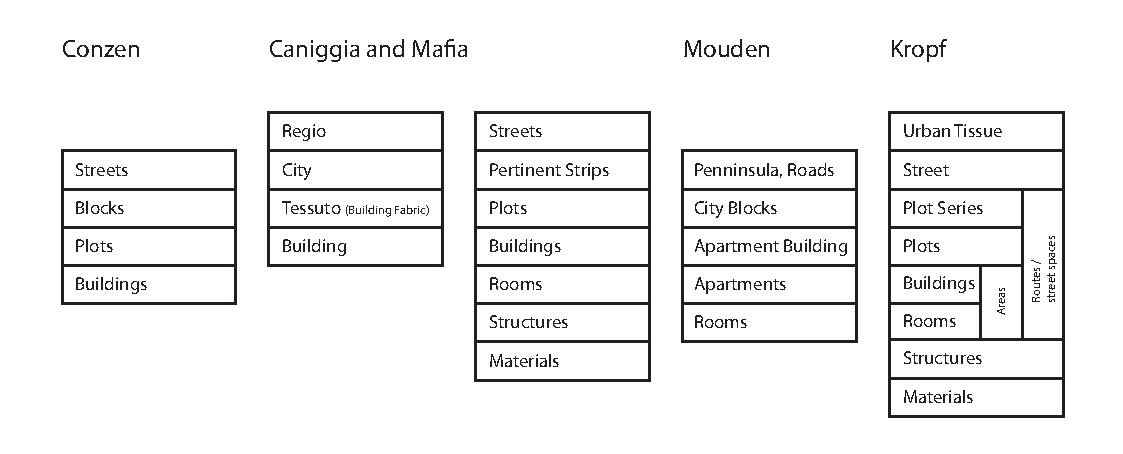
\includegraphics[scale=0.80,page=1]{Images/Typology_Dichtomies.pdf}  
\caption{\bf Different scales of dichotomies. }    
 \label{fig:TypologyDichtomies}  
\end{figure} 

Identifying common patterns is the path towards understanding the formation, evolution and morphogenesis of cities and helps us to understand the underlying mechanism and forces at play. Still, most methods described above require some amount of subjective classification of local input data; the quality and availability of which can vary widely across collection or political districts. Existing empirical methods highlight these mechanisms by evaluating the street network typology\cite{Hillier1989} but neglect their geometrical expanse and neglect their function as places to stay.  A method cannot rely solely on the topology but needs to incorporate the geometry\cite{Louf2014a}. This is why the proposed method uses both size and regularity information within a neighbourhood.  


\subsection{Findings from the application of the methodology.}
The method has shown to be robust and globally applicable in identifying typologies of cities and neighbourhoods. The use of blocks as defined as the space between streets is both universally applicable and shows to have a high information yield. The 2-dimensional representation of this n-dimensional information space shows high potential for further investigations and associations with other indicators of urban activities, human life and economic output.

\subsection{Discussion.}
The method has highlighted that the nature of cities is not unique and that individual neighbourhoods can be compared across continents. The findings also indicate that there is a common structure and that city typologies should be built across cities rather than within, that city centres are more comparable to other centres than to other elements of the same city.
It also allows us now to compare cities on a global scale and investigate further the nature of human settlement. In contrast to previous methods which were limited by the available data from a handful of cities, this method is capable of spanning the globe and can accommodate new datasets as they arise.  


\begin{methods}
%Put methods in here.  If you are going to subsection it, use
%\verb|\subsection| commands.  Methods section should be less than
%800 words and if it is less than 200 words, it can be incorporated
%into the main text.
%
%\subsection{Method subsection.}
%
%Here is a description of a specific method used.  Note that the
%subsection heading ends with a full stop (period) and that the
%command is \verb|\subsection{}| not \verb|\subsection*{}|.




%\section{Methods}\label{sec:Methods}

\subsection{Map imagery sampling.}\label{sec:methods2}
The concept employed in this study was to sample maps of individual city sections, calculate block size and regularity of each section, and then use a self organizing map (SOM) to organise the images into different urban types. 1692 cities with populations greater than 300,000 people\cite{UN2014} were selected for analysis. Map imagery from Google Maps\cite{GoogleStatic2017} was used to provide globally consistent data. 

A two-stage sampling approach was applied to each city. As no standardised urban boundaries are available for all the cities evaluated in this study, a methodology had to be developed to define these. Firstly, a sampling area extending 1.5 km from the identified city centroid\cite{UN2014} was set as a baseline. Then the sampling radius $r$ (km) was scaled, increasing by a power of 0.85 to the proportional increase in population size based on Barthelemy\cite{Barthelemy2016} in 

\begin{equation}
r = \sqrt{ \frac{28.27}{\pi} \left( \frac{p}{300,000}  \right) ^{0.85} }
\end{equation}


Standardising the sampling area in this manner avoided socio-political discrepancies relating to a city's `true' (political) boundary and captured differences in population density and shape between small (e.g., Wellington, New Zealand; Izmit, Turkey) and global mega-cities (e.g., Tokyo, Japan;  Delhi, India). Location sampling areas were adjusted for the earth's curvature\cite{Sinnott1984}. Large water-bodies (e.g., oceans but not coastlines) were removed from the sampling area, as they were not indicative of urban form. 

These procedures result in a population and water body-adjusted circular area centred on the city's central coordinates, capturing the widest extent of each city while minimising the amount of non-urban locations. For example, Figure \ref{fig:parissample} shows the resulting sampling locations used in collecting imagery for Paris. 

\begin{figure}
    \centering    
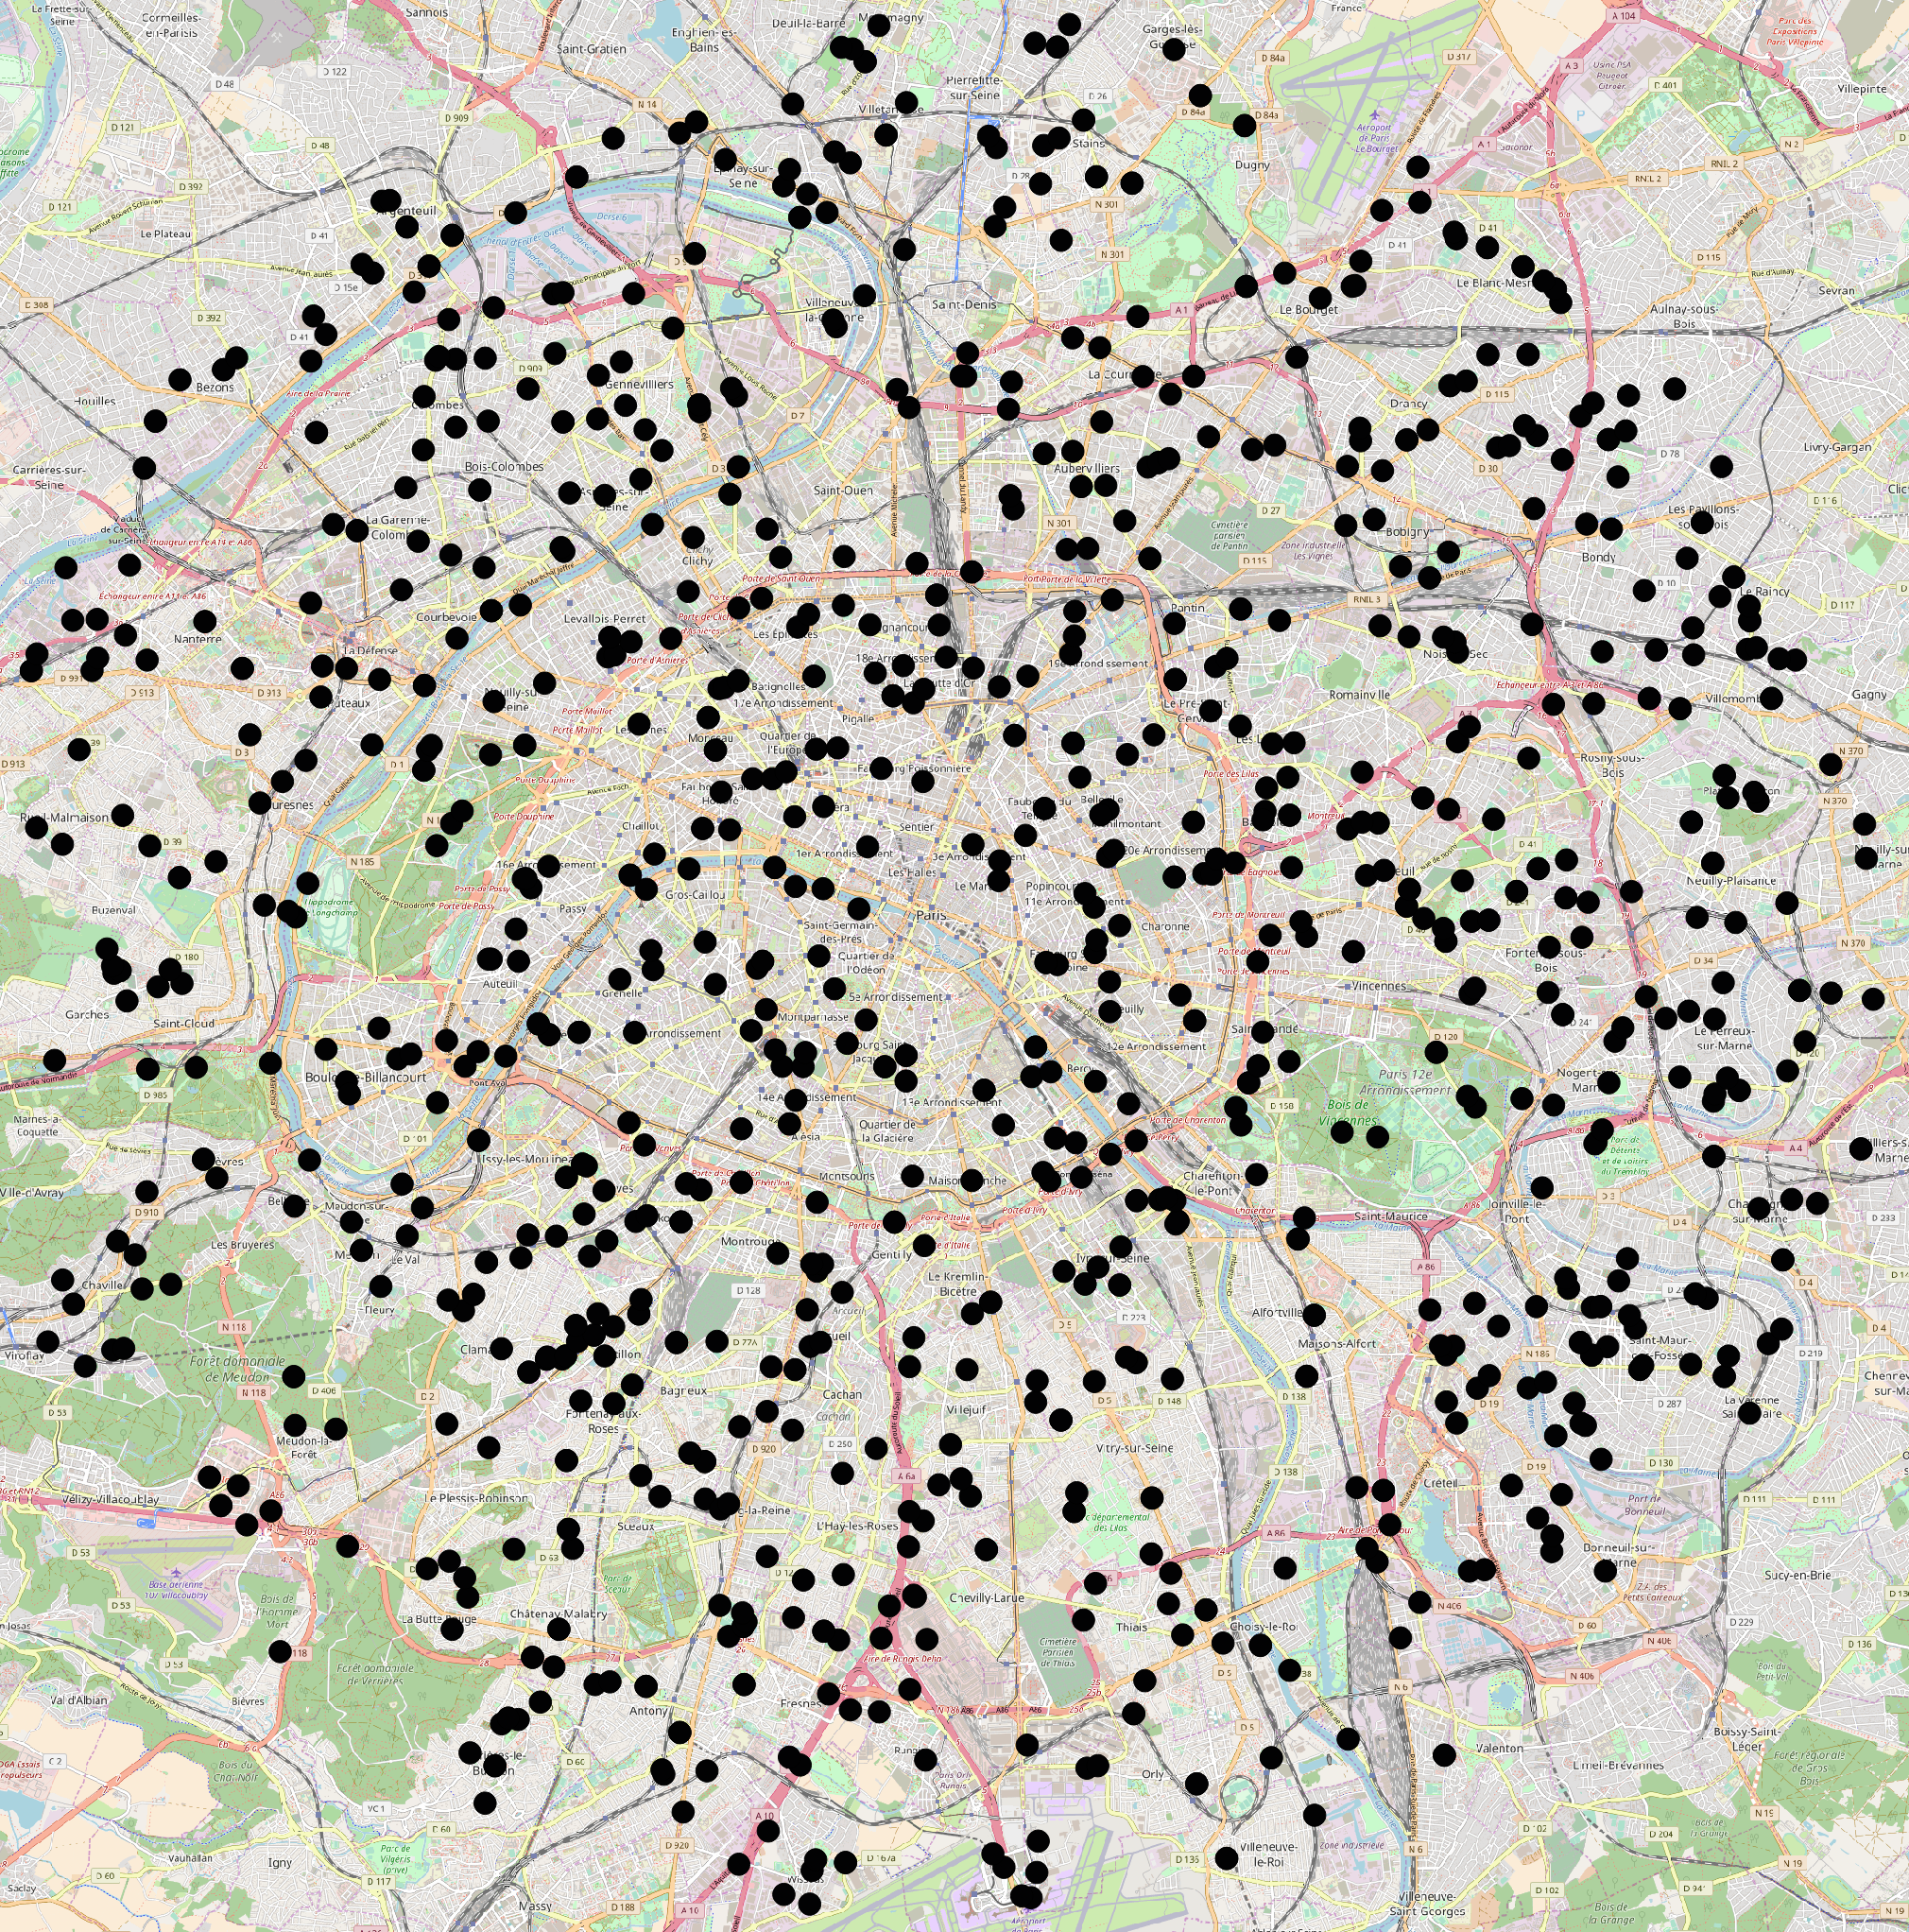
\includegraphics[scale=0.5]{Images/Paris-StreetView-SampleLocations_crop.png}  
\caption{\bf Sampling locations for map imagery (from Paris, France)\cite{GoogleStatic2017}.}    
 \label{fig:parissample}  
\end{figure} 



\subsection{Map imagery source.}\label{methodsimagery}

320x320 pixel sized map images were sampled using a zoom level of 16 (covering 750x750m at the equator and 335x335m at higher latitudes) using a custom style defined with the Google Static Maps API\cite{GoogleStatic2017} (see Figure~\ref{fig:maps} for examples of Paris, France). To ensure each map covers the same area, each image was cropped and resized before processing. The sampled city at the highest latitude was at 64 degrees north, so each image was cropped and resized to include a region of 335x335m. 

The maps provide a high-level abstraction of road (black) and public transport (orange) networks, green space (green), and water bodies (blue). Any remaining space is coded white. Due to mapping inconsistencies in South Korea, all 25 South Korean cities were removed from the dataset, reducing the number of cities to 1667. 1000 maps were sampled per city. In addition, to enable in depth case studies, maps were sampled for Melbourne and Sydney, Australia at a 400m grid resolution across the greater metropolitan areas, resulting in an additional 23,027 locations for Melbourne and 24,596 for Sydney. The total dataset consists of 1,714,591 images.



\begin{figure}
    \centering    
 \includegraphics[scale=0.8]{Images/SampleTraining.png}   
\caption{\bf Four sample Google Maps training data images (from Paris, France)\cite{GoogleStatic2017}.}    
 \label{fig:maps}  
\end{figure} 


\subsection{Calculating block size and regularity.}\label{methodscalc}

Block size and regularity were calculated for each sampled image with the following algorithm, using the Java 8 AWT toolkit\cite{Oracle2018}:

\begin{algorithm}[H]
\SetAlgoLined
\KwResult{Histogram of region sizes and region regularity for an image}
 Using latitude of image sample, determine the number of pixels needed to contain 335x335 meters;\\
 Crop image to this pixel width and height;\\
 Resize image back to 320x320 pixels;\\
 Start at top left point of image;\\
 \While{Locate next white pixel by iterating across rows and columns}{
  Floodfill area using boundaries of all non-white colors (i.e. black roads, green space, blue water);\\
  Count pixel size of region;\\  
  Construct a bounding box of the cloud of points in the region using the Fast Convex Hull algorithm\cite{Javagl2017,GoogleArchive2011};\\
  Count the pixels inside the bounding box;\\
  Use the difference between the bounding box size and the region size as measure of irregularity;\\
  Add size and regularity counts to list for the image;\\
 }
 Sort each list of size and regularity into 15 variable histogram bins;\\
 Combine the two histograms into a single histogram vector to be used in the SOM;\\
 \caption{Calculation of histograms of block sizes and regularity}
\end{algorithm}

Samples of size floodfills and regularity floodfills are shown in Figure \ref{fig:floodfilled}. Sample histograms used in the SOM are shown in Figure \ref{fig:mapsandHist}.

\begin{figure}
\centering    
\includegraphics[scale=0.8]{Images/FloodSample.png}  
\includegraphics[scale=0.8]{Images/FloodfillRegSample.png}     
\caption{\bf Results of flood filled city blocks. (Top) Floodfills of each individual region to determine size. (Bottom) Bounding boxes outlined in red, filled with yellow and count of yellow pixels used for bounding box size. Underlying black outlined regions used for region size.}    
 \label{fig:floodfilled}  
\end{figure} 

\subsection{City size and regularity histograms.}\label{methodshist}

Using the calculated counts, two vectors were constructed for each image, one each for block size and block regularity. The vectors were sorted into 15 histogram bins (the number of bins determined by Sturges' formula\cite{Sturges1926}). To reduce the clumping of data in the first bin, variable bins were used to spread this data across all bins. The first bin starts with a size boundary of 1 and each following bin has a boundary of the current bin boundary times a multiplier. A multiplier of 2.3 was used to fit the maximum count size (320x320 pixels = 102400) into the 15 bins.

The resulting histograms for sample map regions are shown in Figure \ref{fig:mapsandHist}. Histograms input into the SOM were constructed by combining the 15 bins of region size frequencies (on the left side) with the 15 bins of region regularity frequencies (on the right) into a single histogram vector.


\begin{figure}
    \centering    
\includegraphics[scale=0.55]{Images/HistSamples.png}  
\caption{\bf Four samples of map regions (top) and resulting histograms (bottom). Region size and regularity are joined into a combined histogram, with size frequencies on the left side of the graph and regularity on the right.}    
 \label{fig:mapsandHist}  
\end{figure} 

\subsection{Sorting map histograms in the self organising map.}\label{methodscluster}
The self organizing map (SOM) methodology\cite{Kohonen1982} is a data driven technique that transforms a $n$ dimensional data source into a lower dimensional space, commonly a 2-dimensional map, while keeping the relative n-dimensional proximity of two datapoints intact. The distance in the lower dimensional representation is therefore a similarity index, calculated as the euclidian distance, of the higher dimensional space. Each point in the 2-dimensional map has location (x,y) and is associated with a vector of values from the n-dimensional space $(V_{x,y} = [v_{1},v_{2},...,v_{n}])$.

SOM is a generic, objective and robust methodology that has been deployed in many domains and is used for the visualization of n-dimensional data and data exploration\cite{Koleheimen2004}. This methodology was chosen for its ability to create 2-dimensional maps of smoothly changing patterns from the original high dimensional space. Additionally the SOM map spans the extremes observed in the original data and allows for investigation on how the data is distributed, potential paths between two observations or function approximation with non-linear relations\cite{Barreto2006}. 

The 1.7 million maps histograms with 30 dimensions were the initial data space used to train the 2-dimensional SOM (written in Java 8\cite{Oracle2018}). After the randomised initialisation of the 100x100 nodes of the SOM, a random selection of 3.2 million data points from the initial data space were used to transform the 2-dimensional SOM to match it. This iterative process locates nodes that are similar to the training vector and morphs the values of the SOM nodes towards the training values. This training is subjugated to a decay function for both magnitude ($learningDecay$) and  distance ($radiusDecay$) in the SOM, calculated with


\begin{equation} 
radiusDecay = radius * e^{-1 * iteration / timeConstant}
\end{equation}
where $radius$ is $100/2=50$, $iteration$ is the current training iteration (of a total iterations of 3.2 million), and $timeConstant$ is $totalIterations / \log _{10} (radius)$. Learn decay is calculated as
\begin{equation} 
learnDecay = learnRate * e^{-1 * iteration / timeConstant}
\end{equation}
where $learnRate = 0.05$.

After the SOM was trained, each map histogram was classified to find the closest matching node in the SOM. The underlying imagery of the resulting trained SOM was visualised by tiling representative map images from each node x,y point in the SOM in Figure \ref{fig:somresults}. Areas with black have no associated map segments with that particular node x,y location. Most nodes are associated with multiple map segments that have similar characteristics, %(ref{fig:SOM_density.)
Two notable outliers exist that accumulate more than 10,000 map segments (0:21) with 50104 and (6:72) 10723. Both contain map segments that are either only white (0:21) or contain no white (6:72).





The node's x,y locations were encoded into RGB colour codes using a Java 8 port of Color2D\cite{Jackle2017,Steiger2015}. These colours were used in plotting the x,y typologies in qGIS\cite{QGIS2009}.









\end{methods}

%% Put the bibliography here, most people will use BiBTeX in
%% which case the environment below should be replaced with
%% the \bibliography{} command.

% \begin{thebibliography}{1}
% \bibitem{dummy} Articles are restricted to 50 references, Letters
% to 30.
% \bibitem{dummyb} No compound references -- only one source per
% reference.
% \end{thebibliography}

\bibliographystyle{naturemag}
\bibliography{bib}


%% Here is the endmatter stuff: Supplementary Info, etc.
%% Use \item's to separate, default label is "Acknowledgements"

\begin{addendum}
 \item While at the University of Melbourne, Kerry Nice was funded by the Transport, Health, and Urban Design (THUD) Hub.
 \item[Competing Interests] The authors declare that they have no
competing financial interests.
 \item[Correspondence] Correspondence and requests for materials
should be addressed to Kerry A. Nice~(email: kerry.nice@unimelb.edu.au).
\end{addendum}

%%
%% TABLES
%%
%% If there are any tables, put them here.
%%

%\begin{table}
%\centering
%\caption{This is a table with scientific results.}
%\medskip
%\begin{tabular}{ccccc}
%\hline
%1 & 2 & 3 & 4 & 5\\
%\hline
%aaa & bbb & ccc & ddd & eee\\
%aaaa & bbbb & cccc & dddd & eeee\\
%aaaaa & bbbbb & ccccc & ddddd & eeeee\\
%aaaaaa & bbbbbb & cccccc & dddddd & eeeeee\\
%1.000 & 2.000 & 3.000 & 4.000 & 5.000\\
%\hline
%\end{tabular}
%\end{table}

\end{document}
